\section*{Overview}

Parallel binary search is the offline version of ``binary search on answer'' for many queries at once. Instead of
running a separate binary search for every query and rebuilding the data structure every time, it tests all queries at
the same midpoint together, partitions them, and recurses.

\section*{When to Use It}

Use it when:

\begin{itemize}
  \item each query asks for the first time / first index / smallest answer where a monotone condition becomes true,
  \item all updates happen on a timeline or ordered list,
  \item queries can be checked by applying a prefix of updates to some data structure,
  \item the whole problem is offline.
\end{itemize}

\section*{Core Idea}

Suppose updates are numbered \(1 \ldots m\), and query \(q\) asks for the smallest time \(t\) such that
\(\texttt{check}(q, t)\) is true. For one recursion node covering \([L, R]\):

\begin{itemize}
  \item apply updates \(L \ldots M\), where \(M = \lfloor (L+R)/2 \rfloor\),
  \item test every active query at time \(M\),
  \item send satisfied queries left,
  \item send unsatisfied queries right.
\end{itemize}

If going right, many problems let you subtract the contribution already seen in \(L \ldots M\), which keeps the query
state small.

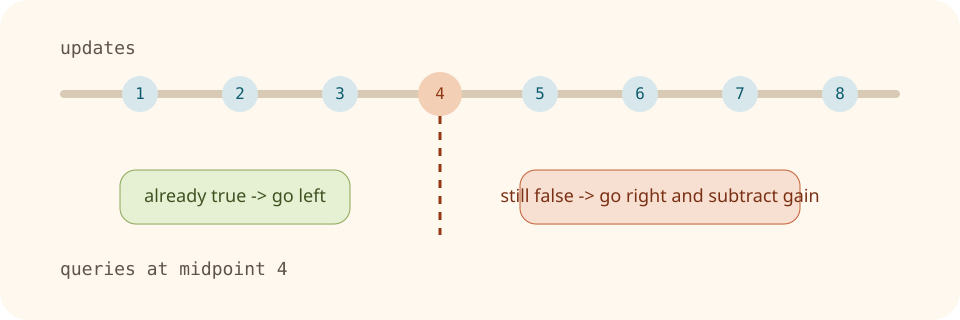
\includegraphics[width=\textwidth]{figures/timeline-batching.svg}

\section*{Key Insight}

The midpoint is shared. That is where the speedup comes from. If \(10^5\) queries all ask for the earliest time when a
Fenwick-tree condition becomes true, you do \emph{one} Fenwick build for the midpoint batch, not \(10^5\) separate
builds.

\section*{Worked Problem}

\paragraph{Problem.}
There are \(m\) positive point updates of the form ``add \(v\) to position \(p\)''. Each query gives \([l, r]\) and a
target \(k\), and asks for the earliest update index after which the range sum on \([l, r]\) is at least \(k\).

\paragraph{Why parallel binary search fits.}
The predicate ``after the first \(t\) updates, range sum on \([l, r]\) is at least \(k\)'' is monotone in \(t\).

\paragraph{Algorithm outline.}

\begin{itemize}
  \item Recurse on update-index intervals.
  \item At midpoint \(M\), apply updates \(L \ldots M\) into a Fenwick tree.
  \item For each query, compute the current range sum.
  \item If the sum is already enough, the answer is in the left half.
  \item Otherwise subtract that sum from the remaining target and continue in the right half.
\end{itemize}

\section*{Correctness Intuition}

Every query keeps an invariant: its remaining target is the amount still needed after all updates strictly before the
current recursion interval have been accounted for. Midpoint testing is therefore exact, and monotonicity guarantees
that the answer lies entirely in one half.

\section*{Complexity Analysis}

If the checker uses a data structure with update/query cost \(T\), then the usual complexity is
\[
O((m + q)\log m \cdot T).
\]
For a Fenwick or segment tree, this becomes \(O((m + q)\log m \log n)\).

\section*{Implementation}

The reference code solves the point-update, range-sum threshold problem above with a Fenwick tree and recursive query
partitioning.

\section*{Common Pitfalls}

\begin{itemize}
  \item Using it on an online problem. The whole method needs all queries in advance.
  \item Forgetting to undo or rebuild the data structure between recursion branches.
  \item Applying it when the predicate is not monotone over the searched timeline.
  \item Mutating the query state incorrectly when moving to the right half.
\end{itemize}

\section*{Variants / Extensions}

\begin{itemize}
  \item Segment tree or DSU based checkers instead of Fenwick trees.
  \item ``First edge when two nodes become connected'' style connectivity queries.
  \item Using iterative bucket rounds instead of recursive divide-and-conquer.
\end{itemize}

\section*{Practice Problems}

\begin{itemize}
  \item Earliest update when a prefix, suffix, or range sum reaches a target.
  \item First time a connectivity or component-size condition becomes true offline.
  \item Batched threshold queries over an ordered stream of events.
\end{itemize}

\section*{References}

\begin{itemize}
  \item \href{https://codeforces.com/catalog}{Codeforces Catalog}.
  \item \href{https://oiwiki.com/misc/parallel-binsearch/}{OI Wiki: Parallel Binary Search}.
  \item \href{https://usaco.guide/plat/parallel-binsearch}{USACO Guide: Parallel Binary Search}.
\end{itemize}
